\documentclass[draftclsnofoot,onecolumn,letterpaper,10pt]{IEEEtran}
\pagestyle{empty}
\usepackage{geometry}
\geometry{textheight=9.5in, textwidth=7in}

\usepackage{float}
\usepackage{graphicx}
\usepackage{algorithm2e}
\usepackage{pgfgantt}

\newcommand{\subparagraph}{}
\usepackage{titlesec}

\titleformat{\section}[block]{\bfseries\Large}{\thesection}{0.4em}{}
\titleformat{\subsection}[block]{\bfseries\large}{\thesubsection}{0.4em}{}
\titleformat{\subsubsection}[block]{\bfseries\normalsize}{\thesubsubsection}{0.4em}{}
\setlength{\parindent}{0pt}
\renewcommand{\thesection}{\arabic{section}}
\renewcommand{\thesubsection}{\thesection.\arabic{subsection}}
\renewcommand{\thesubsubsection}{\thesubsection.\arabic{subsubsection}}



\date{\today}

\title{brew.ai Design Document}

\begin{document}
{\huge\textbf{Senior Software Engineering Design Group 7}}
	\vspace{1cm}

{\Huge\textbf{brew.ai Design Document}}

\vspace{2cm}
\textbf{Connor Yates} yatesco@oregonstate.edu

\textbf{Aravind Parasurama} parasura@oregonstate.edu

\textbf{Cody Holliday} hollidac@oregonstate.edu

\vspace{2cm}
\textbf{Sponsor}

Dale McCauley, College of Business, Oregon State University

\vspace{0.5cm}
	\textbf{Approved:} 

	\textbf{Version:} 1.0


\newpage
\begin{abstract}
	Home beer or mead brewing is not currently a process as simple as brewing coffee.
	We aim to change this, and make home brewing as easy as brewing coffee with the OpenBrew project.
	The OpenBrew project will consist of two major components:
	A hardware system for physically automating the brewing process, and a software system for managing the brewing process, utilizing machine learning 
		to optimize mead or beer recipes.
	Through these components, a user will be able to easily incorporate a fully automated, intelligent home brewing system into an existing setup or 
		as the framework to construct a new brewing system.
\end{abstract}
\newpage
\tableofcontents
\newpage
\section{Introduction}
% Perhaps get rid of these subsection titles, and just combine it into one larger section with appropriate paragraph spacings.
% These talk about the Purpose, scope, etc, of this paper.
brew.ai is a hardware and software solution for automated brewing of mead or beer. Currently, home brewing requires a lot of time, knowledge, and 
	patience. 
As such, it is not accessible to amateurs, and brew.ai attempts to solve this problem. 
From amateurs to professional brewers, we want brew.ai to be useful in automating the brewing process, and helping brewers make better tasting products. 
The brew.ai device itself is a bucket lid that will fit over a brewing device and have various modules incorporated in it. 
The lid device will monitor and control temperature, send and receive commands/data to and from the Android application, and monitor fermentation status.
Improving recipes will take place in the back-end, in the form of a service that the Android software will communicate with. 
As a user, setup will simple and essentially plug-and-play. 
No technical knowledge is needed beyond knowing how to pair a bluetooth bucket lid with an Android device.

\subsection{Purpose}
This document describes the architecture and design of the brew.ai project.
It conforms to the IEEE 1016 System Design Document specification, and lays out the design of hardware, learning, and android interfaces for the project.
By following the designs presented in this document, a technically skilled person or team of people will be able to replicate the prototype we will produce.

\subsection{Scope}
Stated generally, brew.ai is a device which automatically brews fermented drinks and improves its performance over time based on user feedback.
This allows for users who are inexperienced with automated control systems or home brewing to create their own home-brewed fermented drinks.
While brew.ai mainly focuses on home brewing applications, it can theoretically scale to larger applications.

\subsection{Document Overview}
This document is split into three major sections.
The first two talk about the project on a high level, describing who will use the product, what they can do and why they would want to accomplish a goal, and how the system will allow the user to accomplish their goal.
The third major section contains technical design information, to be used by developers to implement the brew.ai prototype.


\section{Glossary}

\section{Stakeholders and Design Concerns}
% Here we list out the design concerns of stakeholders (users, etc...) that we address in this document.
% By laying out the design concerns now, we can address each in turn in the subsequent design sections.
While the design team and sponsor are direct stakeholders of this project, they do not have any concerns, apart from technological feasibility, that impact the design of the product.
Rather, the eventual users are the stakeholders whose requirements influence the final design of the product.

There are three major design concerns when viewing this product from the viewpoint of the user.
First, the brewing system must be able to learn from past trials, based on user feedback. 
This design concern is addressed in Section~\ref{sec:learning}.
Secondly, the system must automate the brewing process. 
This design concern is addressed in Section~\ref{sec:hardware}.
Finally, the user must have a method of interacting with the brewing device, to measure progress and see how the system is performing.
This is addressed in Section~\ref{sec:android}.
While these design concerns are broad, when put together they describe the basis of the project.

\section{System Overview}
In order to satisfy the three major design concerns, this project is cleanly divided into three respective technological sections.
These technological sections are self-contained, except for data messages which must be shared intermittently.
This section provides a brief overview of these sections, and describes the method by which they will communicate.

To implement the intelligent learning, a standard reinforcement learning agent will be created, and will be able to communicate with both sections.
Hardware will be created to solve the task of automated brewing, and will communicate exclusively with the intelligent agent.
A user interface will be created on an dedicated platform, which will communicate with the intelligent agent.
In this design, the intelligent agent can act as the translator between the hardware and user interface.

\subsection{Data Design}
The messages passed between the hardware, agent, and interface are described in this section.
All three sections must be able to transmit and receive specific message types.
The hardware must continually pass current sensor readings to the intelligent agent.
These sensor readings will be communicated as a byte stream, since they are nothing more complicated than a few numbers.
The hardware must be able to receive action requests from the agent.
Action requests will be sent as a status number, signifying which of the three actions described in Section~\ref{sec:learning} the hardware should take.
The user interface will need to communicate basic user requests to the intelligent agent.
Some of these requests, such as an emergency stop, will not take part in the learning process.
Rather, they are passed to the agent module because it already contains this level of functionality, as seen in Section~\ref{sec:learning}.
The user interface will also need to communicate the user's satisfaction to the learning agent.
This message will take part in the learning process, but is not necessary for the learning agent to have until after the batch is completed.
Finally, the user interface needs to receive the current status of the brewing process.
This information, which encompasses elements such as runtime, temperature, and estimated completion time, will be sent in the JSON format.

The dataflow diagram in Figure~\ref{fig:dataflow} summarizes the internal message passing in the brewing system.
\begin{figure}[h]\label{fig:dataflow}
\begin{center}
	\caption{Dataflow Between the Three Major Components}
	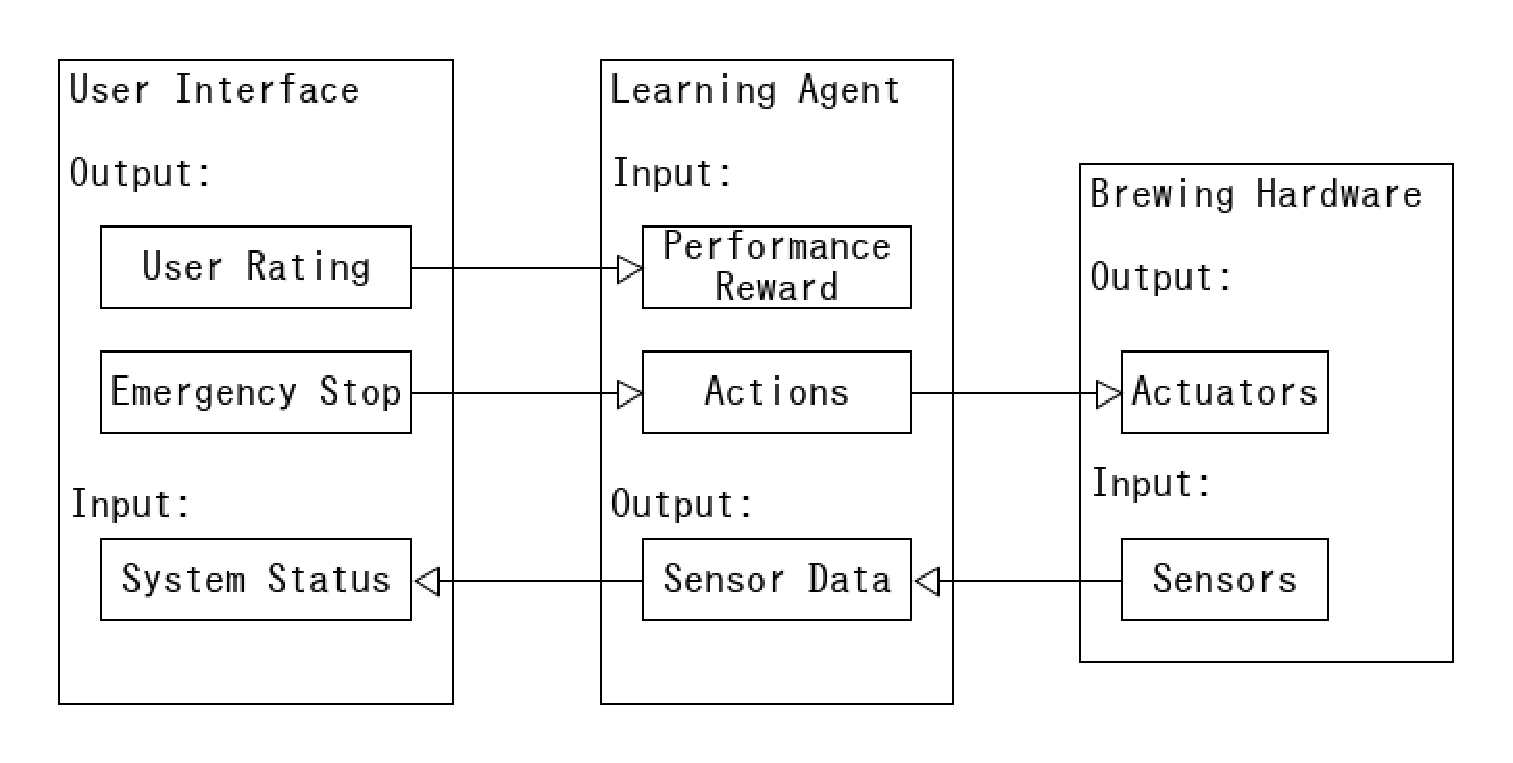
\includegraphics[width=\linewidth]{dataflow.eps}
\end{center}
\end{figure}

\section{Design Viewpoints}
% Details each design point we choose for this project.
% The tech review had 3 technologies, with 3 choices/investigations for each tech.
% Each of the three technologies chosen should be designed in detail in its own "viewpoint".
% each viewpoint then has its own "view". There can be more than one of these.
% the views describe the specific implementations that each viewpoint covers. Refer to the doc for more info.

\subsection{Abstract Learning from Previous Trials}\label{sec:learning}%connor's
From the inception, a major component of this project is the idea that it can learn from mistakes and experiments, and improve the quality of the brew over time.
This section looks at the system design from the viewpoint of artificial intelligence creation.
From this perspective, all other design choices of the project are abstracted into general data sources and sinks.
To further illustrate this point, the view Impact on Other Designs, in Section~\ref{sec:AIImpact}, will introduce the reader to this viewpoint by describing its view of the rest of the system.
From there, the AI system's internal view of the brew.ai system will be explained and designed.

\subsubsection{Impact on Other Designs}\label{sec:AIImpact}
From the viewpoint of learning, the two other major viewpoints, electronic hardware and user interfaces, have little to no impact upon the operations of the system.
There will be interaction between these viewpoints, but that does not imply the other sections will autonomously impact the operation of the system.

From the AI perspective, the system is built as a thinking agent, with the ability to send and receive signals.
This allows the agent to change the world it sees (input signals) through its actions (sent signals).
The hardware will be the main component the AI will interact with, as it provides information about the world through sensors, and can change the world through its actuators.
From this perspective, the hardware is generalized into the two categories: sensors and actuators.
This is a common view for an agent to take in regards to its interaction with the world~\cite{RussellNorvig}.
A diagram summarizing the agent's view of the system is presented in Figure~\ref{fig:AIsystemDesign}.

\begin{figure}[h]\label{fig:AIsystemDesign}
\begin{center}
	\caption{brew.ai System Hierarchy from the viewpoint of the agent}
	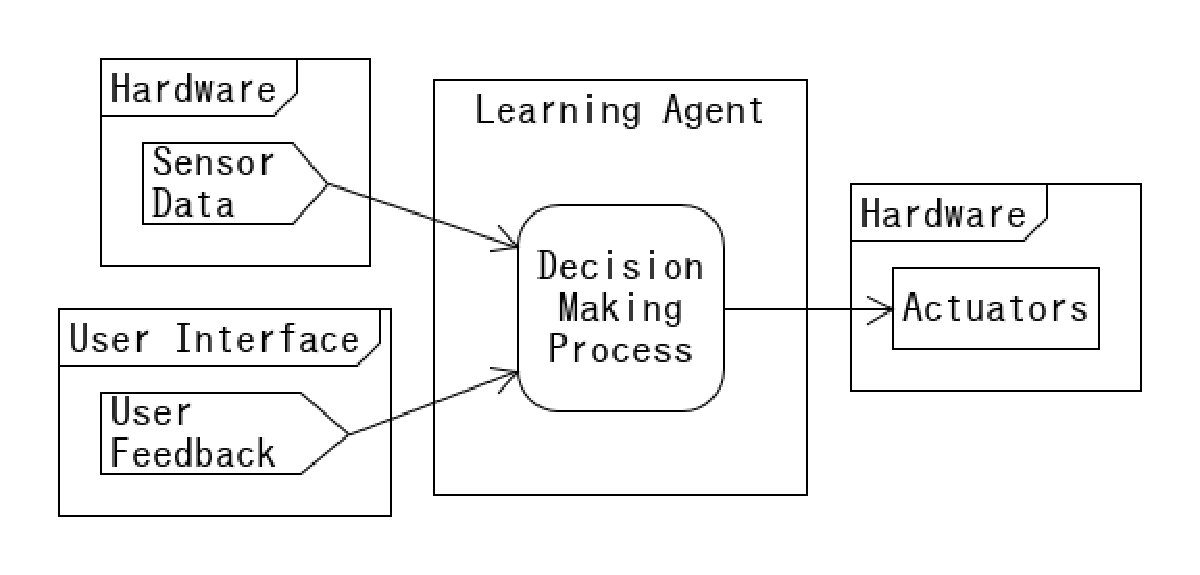
\includegraphics[height=18em]{highView.eps}
\end{center}
\end{figure}

The agent will also view the user interface as source of actuators and sensors, but this will be limited in scope.
The main task of the agent is to brew drinks, not report information to the user.
Therefore, the main decision-making processes will focus on the hardware interaction (reading sensor values, changing temperature levels, etc.) and not on intelligent interaction with the user.
The direct interaction between the user and the AI will be limited to sending statistical information for display, and basic controls such as start-stop controls.

A standard communication layer will be necessary to communicate between the AI, hardware, and interface.
This will be implemented with standard protocols and library packages, such as JSON for interface communication, and byte streams for hardware interaction.
Builtin Python libraries exist for these communication protocols, and subsequently will be used.

\subsubsection{Learning Algorithm} 
% talk about what algorithm I chose.
% Any design considerations that this algorithm requires
% design of this piece, in the context of the project
The agent will be using standard Q-learning, as it provides a proven framework for creating intelligent agents that can learn with delayed rewards~\cite{SuttonBarto}.
This is applicable to our problem since the main reward signal (the input from the user) is not available until the brewing process is complete.

The standard Q-learning algorithm requires a set of states $S$ and a set of available actions $A$.
By performing an action $a_t$ from $A$, the agent is able to change the current state $s_t$.
The Q-table comes into play by learning which action is the best action to take when the agent is in state $s_t$~\cite{SuttonBarto}
The central idea of the algorithm is the value iteration update, defined in Equation~\ref{eq:Q(s,a)}
\begin{equation}\label{eq:Q(s,a)}
	Q(s_t,a_t) \leftarrow Q(s_t, a_t) + \alpha \cdot \left( r_{t+1} + \gamma \cdot \max_a Q(s_{t+1},a) - Q(s_t,a_t) \right)
\end{equation}

Any given state $s_t$ will be composed of the following information:
\begin{itemize}
	\item A numerical signal from the thermocouple
	\item A numerical signal from the carbon dioxide sensor
	\item A numerical signal from the digital hydrometer
	\item A numerical signal representing the current runtime of the brewing process
\end{itemize}
The first three signals come from sensors present in the brewing setup, which will allow the agent to perceive how the current brewing process is proceeding.
The last signal will help the agent differentiate between the start and end of the brewing process, to help differentiate between potentially similar looking states which may require different responses.
The state will be composed as a linear array of this information.
At time $t$, the state $s_t$ will be defined as
\begin{equation}
	s_t = \langle T_t, C_t, G_t, t \rangle
\end{equation}
The units and order of magnitude of the first three signals will be kept at the sensor defaults.
The time dimension will be provided in hours, represented as a floating point number to allow for sub-hour accuracy.

There are three available actions for the agent to choose from.
Two are based on actuators in the brewing setup.
These actuators are a submersible heating element, and a motor controlled stirring mechanism.
The agent can control the power state of the heating element, and the power state of the electric stirrer.
Additionally, the agent can take an action to signal that the brewing process has completed, bringing the process to an end.

\subsubsection{Decision Making Structures}
An important aspect of intelligent decision making is the computational structure which allows for decisions to be made.
Neural networks are a classic method of non-linear function approximation~\cite{RussellNorvig},  which we will use to approximate the Q-table.
This can be done by collapsing the state into a single dimensional vector, and using this as the input to the neural net.
The neural net will output the Q-value associated with each action for this state, which are used by the Q-learning as normal, if they came from a Q-table.

The neural network will take as input the state $s_t$, and output Q values for each associated action.
It will have at least 1 hidden layer residing between the input and output layers.
An example neural net structure is given in Figure~\ref{fig:nn}.

\begin{figure}[h]\label{fig:nn}
\begin{center}
	\caption{Proposed Neural Network Structure}
	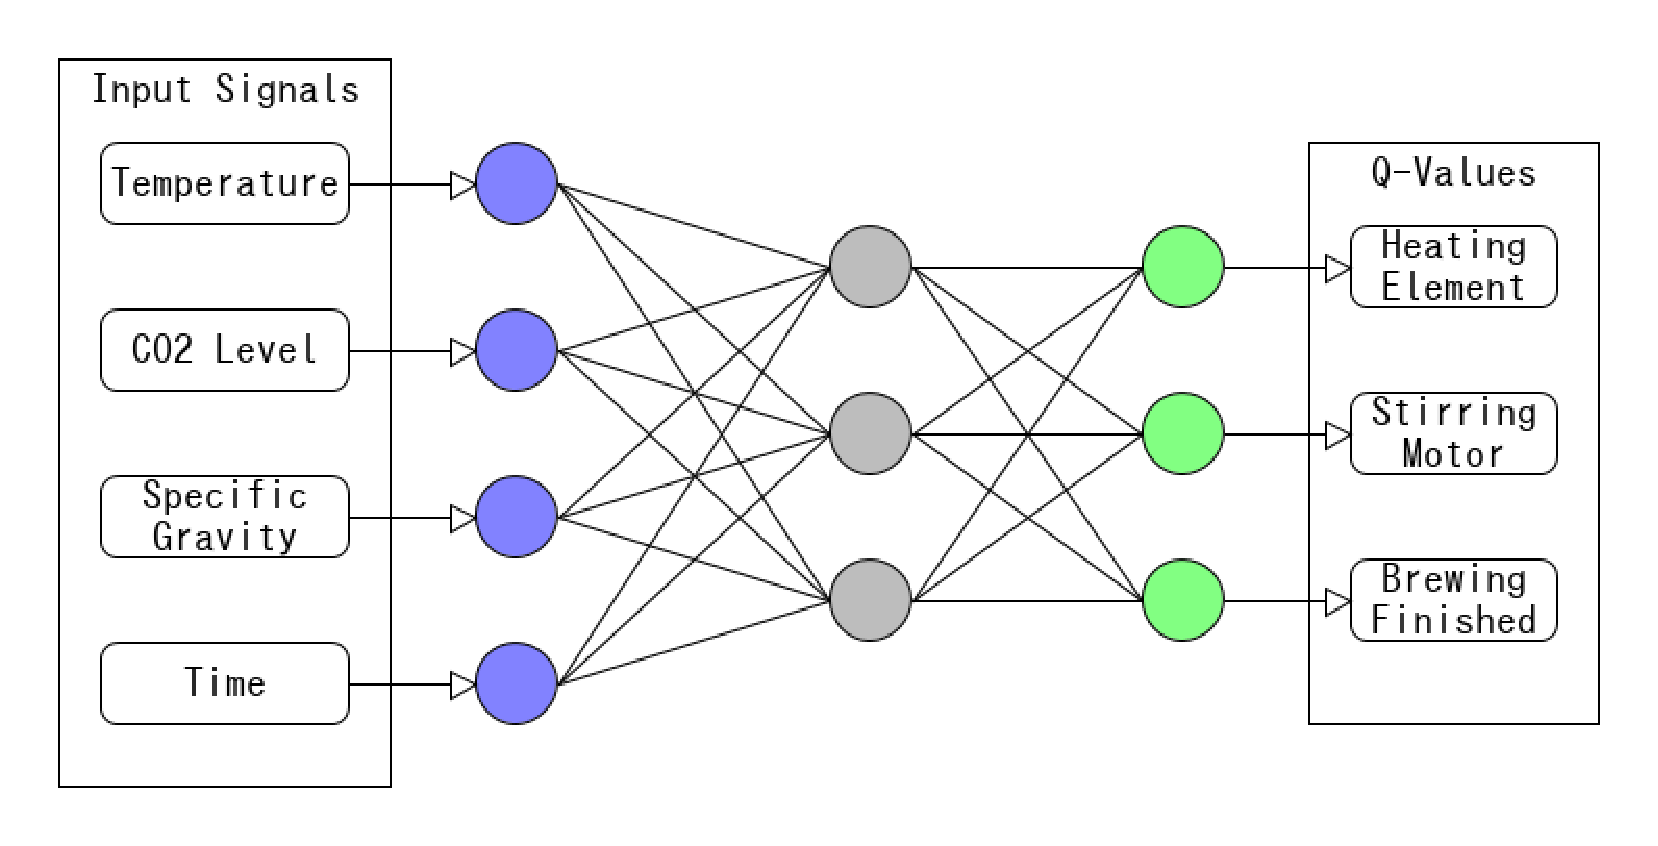
\includegraphics[width=\linewidth]{nn.eps}
\end{center}
\end{figure}

In order to train the neural network to approximate the Q-table, backpropagation will be used along with a sum-of-squares loss function.
Methods such as backpropogation are standard entries in neural-network and machine learning libraries, which we will use to provide the implementation.

If the neural network structure does not provide reliable performance, then we will use a traditional Q-table to implement the learning.
The reason this is not used by default is because we have a continuous state space, which cannot be contained in a finite table.
However, by observing the incoming data, we can provide an encoding scheme which will map the continuous domain of data inputs into a finite, discrete set which can be used to construct the table.

\subsubsection{Overall Agent Structure}
Combining the ideas from the previous sections, the learning agent is summarized as follows, both in diagram and paragraph.

\begin{figure}[h]\label{fig:AgentStructure}
\begin{center}
	\caption{Agent structure, showing learning functions, neural network, and data insertion points}
	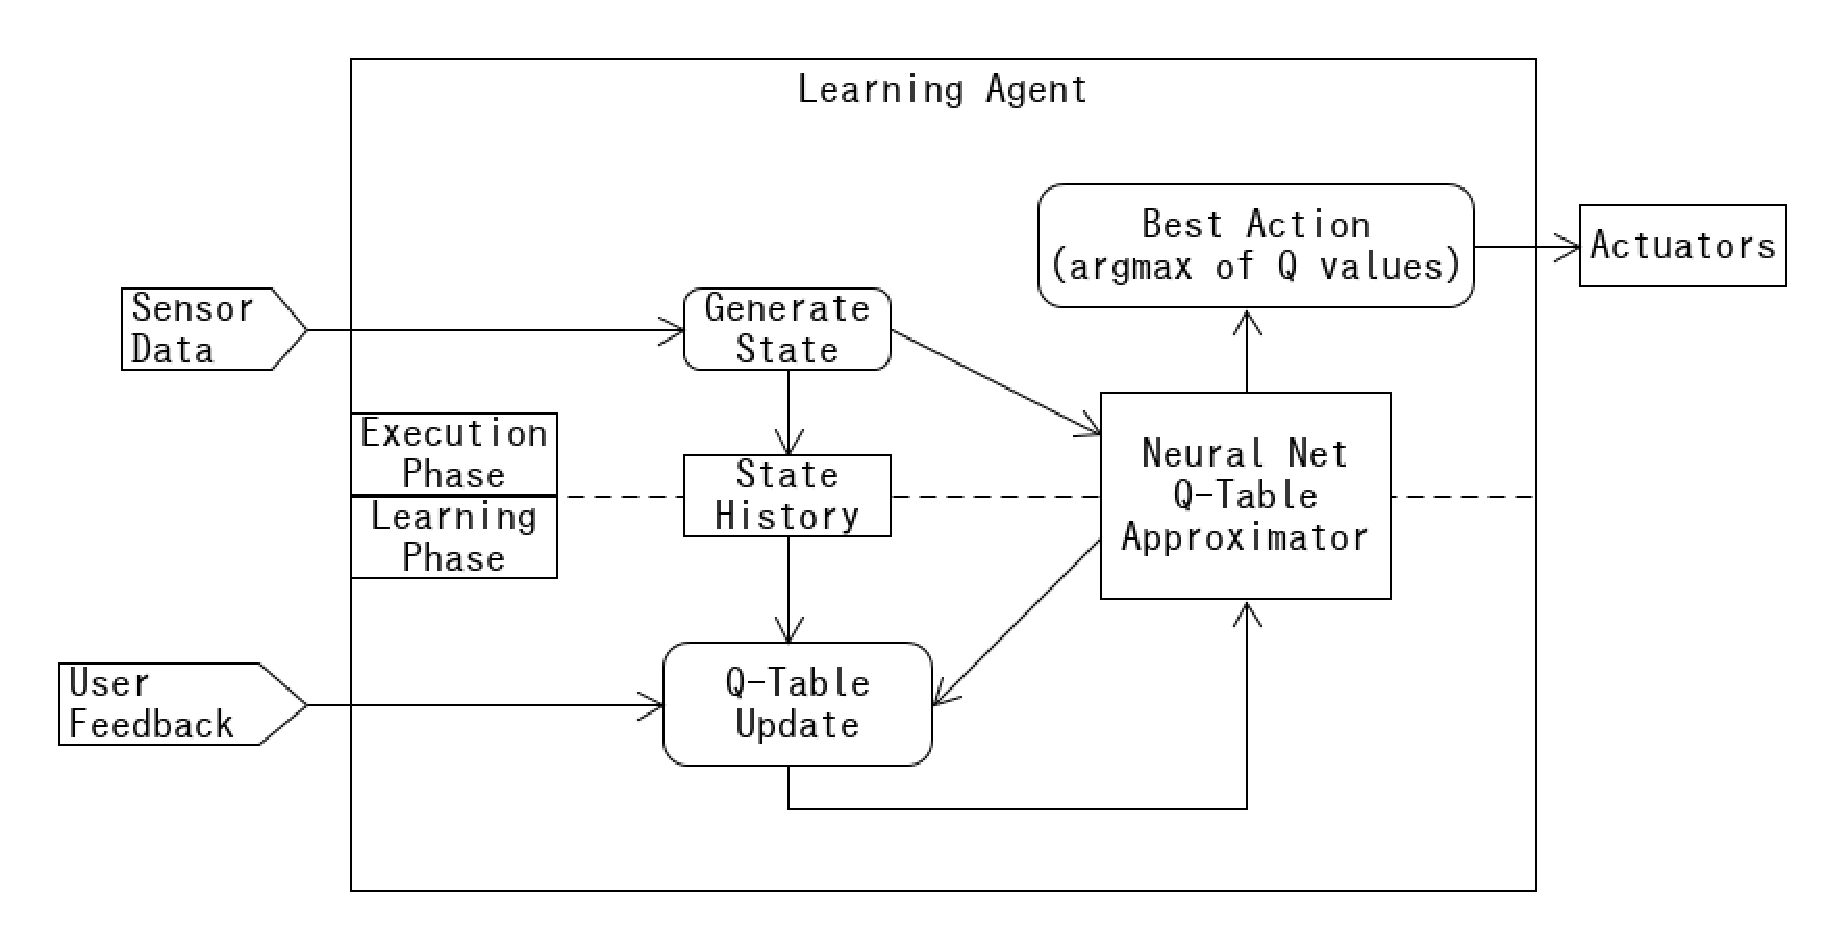
\includegraphics[width=\linewidth]{totalagent.eps}
\end{center}
\end{figure}

A neural network, composed of an 4-dimensional input layer, one or more hidden layers, and a 3 dimensional output layer, will be used as the approximate Q-table.
Input signals will be generated by the microcontroller in direct control of the brewing setup, and combined into the state the agent perceives.
The agent will take actions by taking the action associated with the maximum Q-value at time-step $t$.
These actions will be sent to the microcontroller, where they will be used to control the state of the brewing process.
It will learn by using the Q-learning iterative update function (Equation~\ref{eq:Q(s,a)}), and receiving its reward from the user.


\subsection{Android-Based User Interface Design}\label{sec:android}%cody's
\subsubsection{Interface Device}
The device chosen for the user interface was the Android device.
Android has a well-used set of tools and a huge community for development, which is why it is the best choice.
IDEs like Android Studio are continuously developed to support third party development \cite{AndroidStudio}.
In addition, Android devices can be found at a reasonable price.
The average Android device in 2014 was around \$250 \cite{AndroidStats}, but the Blu Stduio X8 HD is available for \$49.99 as of November 30, 2016 \cite{BluStudioX8}.
The screen is 5 inches from corner to corner, which provides enough space to have many options or buttons on screen.
Our choices are not limited to one device, since there are many other phone manufacturers that produce Android devices.

Choosing the Android as the user interface device determines how the interface is implemented.
Android uses XML for the design and Java for functionality.
Other options are available for programming an Android App, but they are mostly for developing videogames \cite{Pygame}.
Our goals only involve a simple button interface as well as graphical display of data.
Android also offers special libraries that enable native graphing on the device. 
The choice of interface device also affects how the Controller interacts with the interface.
Rather than just being a display for the controller, the Android will have to implement protocol to interact with the controller so that there is a logical flow of data and control.
The data flow between the Android and the controller will be implemented using a TCP connection rather than designing our own message protocol.

\subsubsection{UI Connection to controller}
A USB connection to the controller was determined as the best option for this project.
A simple method of interfacing the Android to the controller is using an Android Debug Bridge \cite{ADBDOCS}.
The Android Debug Bridge is a program that  allows an Android device to be controlled via the command line.
The command line tool allows a PC to manage app installation and activity, as well as file transfers to the device from the PC.
ADB can be installed on a Raspberry Pi, so there are no inherent issues with compatibility \cite{ADBPI}.
To transfer data from the controller to the Android, the controller can just use the ADB command line tool to send the data as a file to the device.
The ADB also allows for port forwarding, so the Android device will communicate with the controller via a TCP connection.
The simplicity of this interface allows for more complex control mechanisms between the controller and the interface as well as leaves room for design improvements.

The controller will have a Python program running that will interact with the Android device using a combination of sockets and bash scripts.
The sockets will be used for control mechanisms, such as starting the brewing process, and the bash scripts will be used as a method for sending data.
Data from a batch is sent from the controller to the Android as a file so that the Android can graph the data locally.
The commands to send the data will live in bash scripts that will be called by the Python program.
Any images that need to be generated on the controller can be sent to the Android via ADB as well.
Physical advantages of a USB connection include preventing loss of data due to interference or connection issues as well as reduce the number of connections on the power supply.


\subsubsection{Dataflow to UI}
The path the data will take is through the controller to the user interface for analysis.
The interface will receive a copy of the data after it is sent to the controller from the microcontroller.
The controller will format the data into a JSON file using the built in JSON Python library \cite{JSONPython}.
The controller will send a JSON file of the data view the ADB command line interface.
After the user interface receives the data, it will turn the JSON file into an object that it will then use to graph the data.
The analysis will take place in the Android app and take place in an asynchronous thread, to prevent the main thread from locking up the interface.
The thread will use a library called Graphview to graph the data on the device. \cite{Graphview}

Graphing on the Android device will reduce the amount of processing that takes place on the controller.
The processing on the controller should be limited to reinforcement learning and data transfer.
However, data transfer and analysis will not take place at the same time on the controller, so there is not a problem with resource sharing, but there is a worry of long term wear and tear.
The brewing device is a long term solution to the homebrewing problem, so we need to maximize the life of the device.
To prevent premature loss of a CPU, the processing load will be spread out over both the controller and the user interface device.

\subsection{Brewing Hardware and Electronic Controls}\label{sec:hardware}%aravind's section
The brewing hardware is expected to perform the commands received from the Android client, while also automatically managing
some basic regulation functions on its own. The hardware will collect data about the brewing process and relay that back to the
Android application.

\subsubsection{Temperature control implementations}
For temperature control, an electric immersion heater will be used.
Immersion heaters are ideal as they can hang from the lid assembly and by submerged into the water. \cite{immersion}
These heaters will provide quick and reliable heating for large quantities of liquid, and this functionality is exactly what is needed for this purpose.
The immersion heater will need to be powered externally to the microcontroller, however control signals for the device must come from the
	microcontroller.
Some kind of power supply or H-BRIDGE module may need to be built to facilitate the power of an immersion heater.

\subsubsection{Data collection from brewing process}
For data collection, an array of sensors has been chosen:
\begin{enumerate}
	\item A thermocouple, for minimal calibration temperature data gathering \cite{thermocouple}. Thermocouples are advantageous over other 
		temperature modules as these are more accurate, and require no tuning with the microcontroller's ADC.
	\item A carbon dioxide sensor, for measuring current fermentation levels by performing calculations versus the initial gravity.
	\item A digital hydrometer for measuring initial gravity \cite{makingmead}.
\end{enumerate}
\subsubsection{Hardware connection to the client}
Data will be transmitted to the front-end by means of bluetooth. A bluetooth module will be used that supports interfacing directly with AVR's
USART functionality. This bluetooth module should easily pair with the Android application and transfer data. Any direct data pipeline to the service
will need to be its own physical UART connection, for which the standard ATmega32u4 USART should suffice \cite{datasheet}.

\subsubsection{Central control system}
To bring all of the hardware components together, we will be using the Teensy 2.0, powered by the ATmega32u4 \cite{teensy}.
This microcontroller allows for basic routines to be performed, and has a variety of hardware functionality that will be extensively used in this project.
For instance, USART will be used for data transfer, the ADC will be used to read any voltage and temperature if using a thermistor.

\section{Design Rationale}
Remove?

\section{Testing Details and Timeline}
% Reuse gantt chart for project timeline, and specify where testing would take place in that chart.
% Add details for testing your own components, and potentially testing interactions with other components.
Testing will be incorporated into the each of the prototype iteration stages as desribed below: \\
\begin{ganttchart}[
    y unit title=0.5cm,
    y unit chart=0.6cm,
    time slot format=isodate-yearmonth,
    compress calendar,
    title/.append style={shape=rectangle, fill=black!10},
    title height=1,
    bar/.append style={fill=green!90},
    bar height=.6,
    bar label font=\normalsize\color{black!50},
    group top shift=.6,
    group height=.3,
    group peaks height=.2,
    bar incomplete/.append style={fill=green!40}
  ]{2016-10-27}{2017-05-02}
  \gantttitlecalendar{year} \\
  \gantttitlecalendar{month} \\
  \ganttbar{Requirements Document}{2016-10-28}{2016-11-04} \\
  \ganttlinkedbar{Survey Potential Users and Customers}{2016-11-04}{2016-11-19} \\
  \ganttlinkedbar{Develop Lean Canvas Model}{2016-11-20}{2016-11-27} \\
  \ganttlinkedbar{Research AI, ML, RL structures}{2016-11-04}{2016-11-24} \\
  \ganttgroup{Construct Prototype}{2016-11-04}{2016-12-19} \\
    \ganttbar{Hardware}{2016-11-04}{2016-11-05} \\
    \ganttbar{Electronics}{2016-11-05}{2016-11-10} \\
    \ganttlinkedbar{Gather Data}{2016-11-10}{2016-12-05} \\
    \ganttbar{Construct Control Policy}{2016-12-05}{2016-12-19} \\
    \ganttbar{Gather More Data}{2016-12-19}{2017-01-19} \\
    \ganttlinkedbar{Second survey of users}{2017-01-19}{2017-01-26} \\
    \ganttlinkedbar{Update Lean Canvas Model}{2017-01-26}{2017-01-29} \\
  \ganttgroup{Second Prototype Iteration}{2017-01-19}{2017-03-04} \\
    \ganttbar{Assemble Hardware}{2017-01-20}{2017-01-21} \\
    \ganttlinkedbar{Electronics}{2017-01-21}{2017-01-26} \\
    \ganttbar{Gather Data}{2017-01-26}{2017-02-19} \\
    \ganttbar{Rework Control Policy}{2017-02-19}{2017-03-14} \\
    \ganttbar{Prepare For Expo}{2017-03-14}{2017-04-29}
\end{ganttchart}

Testing for the hardware implementation and the learning service will be a matter of ensuring full functionality at every stage, and then
	subsequently improving upon the implementation over time.
Unit testing is only relevant to the Android interface, as there are various functions and user edge cases to be considered when testing individual 
	components.
While working on gathering data and constructing/improving control policy for both prototype iterations, testing for the Android client will 
	take place, both in the form of individual user feedback, but also unit testing of specific software functions.

\section{Summary}
This document provided the in-depth discussion and design of the three main project ares highlighted by previous work.
Hardware, an intelligent learning agent, and an android interface will be combined to create the brew.ai project.
By following the designs detailed in this document, the project will transition from an idea into reality.

% References
\bibliography{design_document}
\bibliographystyle{ieeetr}


\end{document}
